\section{Anwendungsfälle}

\subsection{Scatterplot}

Der erste Anwendungsfall soll die Einordnung von Ländergruppen zum Happiness Score und eventuelle Mustererkennung ermöglichen. In Abbildung \ref{fig:scatterplot_anw} ist die Standard Konfiguration des Scatterplots abgebildet. Diese sieht der Nutzer wenn er die Visualisierungsseite aufruft. Hier werden die Dimension Happiness Score und Life expectancy gegenübergestellt. Die Ländergruppen sind farblich in der Legende über dem Plot zugeordnet.\\

\begin{figure}[h]
 \centering
 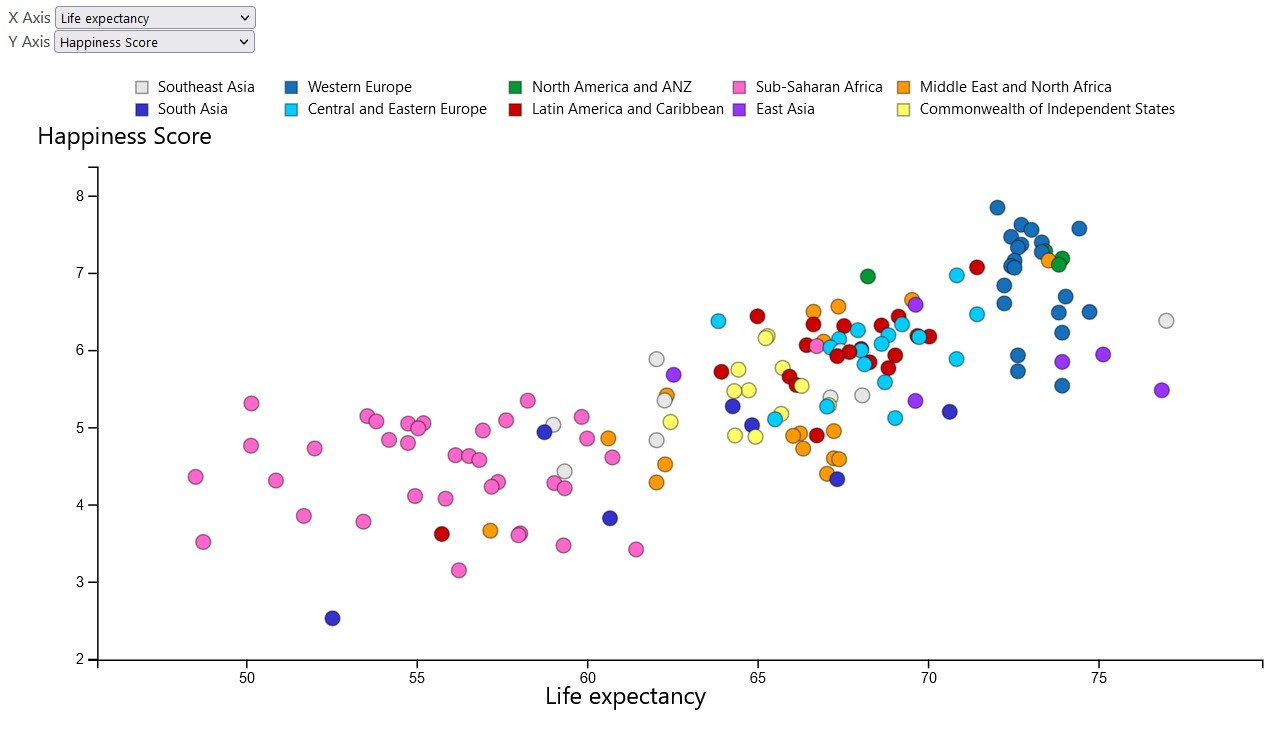
\includegraphics[width = \textwidth]{img/scatterplot_anw.jpg}
 \caption{Scatterplot Anwendungsfall}
 \label{fig:scatterplot_anw}
\end{figure}

Der Nutzer kann auf dem Plot eine Idee davon bekommen in welchen bereichen der Happiness Score Verteilung die Länder der einzelnen Regionen sich befinden. So sind die meisten Länder aus Westeuropa bei ca. über 6 Punkten und solche aus Sub Sahara Afrika bei unter 5.5 Punkten. \\

Auch ungefähre Zusammenhänge, also Korrelationen, lassen sich hier visuell leicht erkennen. Alle Punkte befinden sich auf einem aufsteigenden Korridor von der linken untern zur rechten oberen Ecke. Eine höhere Lebenserwartung Korreliert also positiv mit einem höheren Happiness Score. Eine genaue Korrelation lässt sich nicht visuell bestimmen, dies ist aber auch nicht der Anspruch. \\

\subsection{Polarplot}

Im zweiten Anwendungsfall geht es darum alle Informationen über ein Land zu erhalten. Viele Nutzer wird es interessieren was die Statistiken zu ihrem Land sind. Der Scatterplot ermöglicht es zwar die Ländernamen herauszufinden, aber es wäre viel aufwand ein bestimmtes Land unter all den angezeigten Punkten zu finden. Daher gibt es im Polarplot ein zugehöriges Dropdown Menü mit dem man ein Land aussuchen kann. Das verwendete HTML Element ermöglich es auch dieses zu durchsuchen. Klickt der Nutzer also das Dropdown an und beginnt dann seinen Landesnamen einzutippen wird das Dropdown das entsprechende Land anzeigen. \\

\begin{figure}[h]
 \centering
 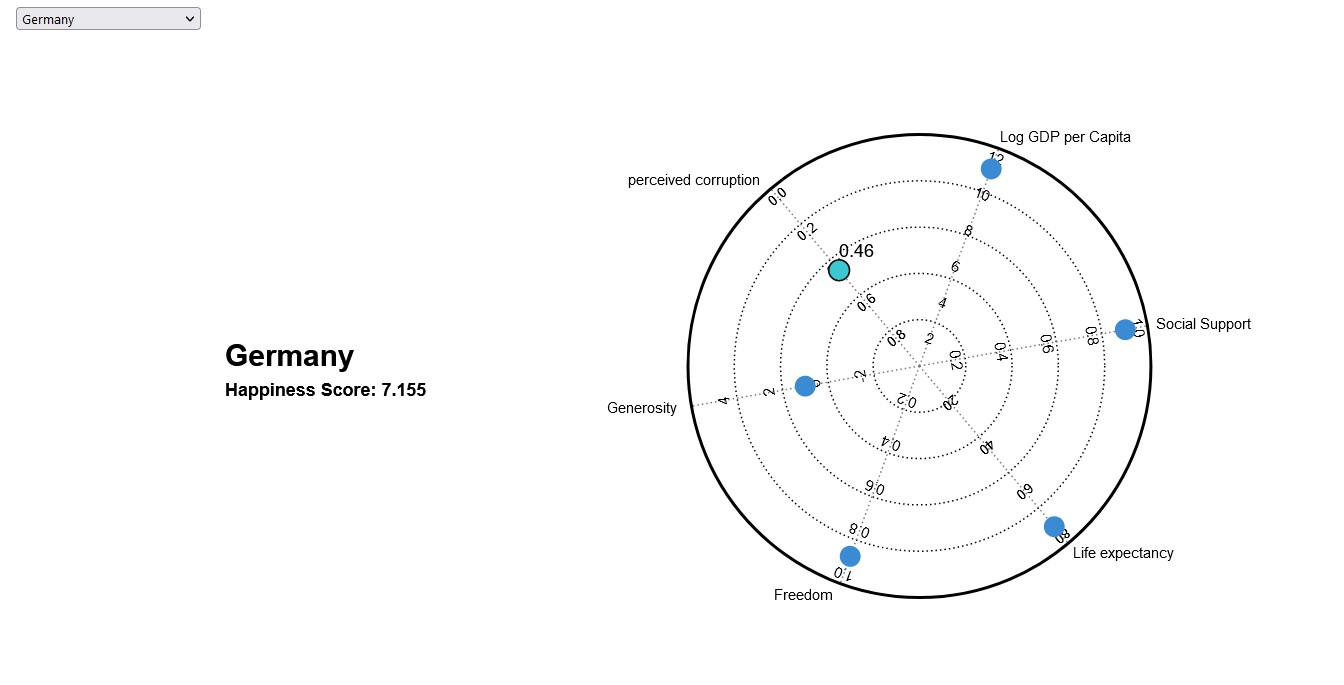
\includegraphics[width = \textwidth]{img/polarplot.jpg}
 \caption{Polarplot}
 \label{fig:polar_example}
\end{figure}

In Abbildung \ref{fig:polar_example} wurde Deutschland als Land ausgewählt. Nun sind alle Größen über DEutschland für den Nutzer sichtbar. Der Happiness Score wird unter dem Landesnamen angezeigt, während die restlichen Größen sich im Polarplot befinden. Das Zielscheibenartige Layout macht es recht einfach die Position der abgebildeten Punkte schnell wahrnehmen zu können. \\

Hier sind die Daten auch nach den entsprechenden Skalen angepasst. Variabeln welche mögliche Werte von 0-1 haben werden hier auch auf einer Skala von 0-1 eingetragen. Solche die kein theoretisches Maximum haben bekommen einen Maximalwert der nahe dem größten Wert aus dem Datensatz ist. Dies ist ein Unterschied zur Skalierung im Scatterplot, welche dynamisch stattfindet um möglichst viel des Plots mit Daten zu füllen und Muster so sichtbarer zu machen. 

\subsection{Zeitreihe}

Die Zeitreihen Visualisierung soll dazu dienen die Werte in historischen Kontext zu stellen und Entwicklungen der einzelnen Länder sichtbar und Vergleichbar zu machen. Der Nutzer wird sich vermutlich dafür interessieren wie sich sein eigenes Land entwickelt hat und wie es im Vergleich zu anderen Ländern dasteht. Diese Ansprüche deckt diese Visualisierung ab. Es ist möglich die Stetigkeit der Entwicklung eines Landes nachzuvollziehen.\\

\begin{figure}[h]
 \centering
 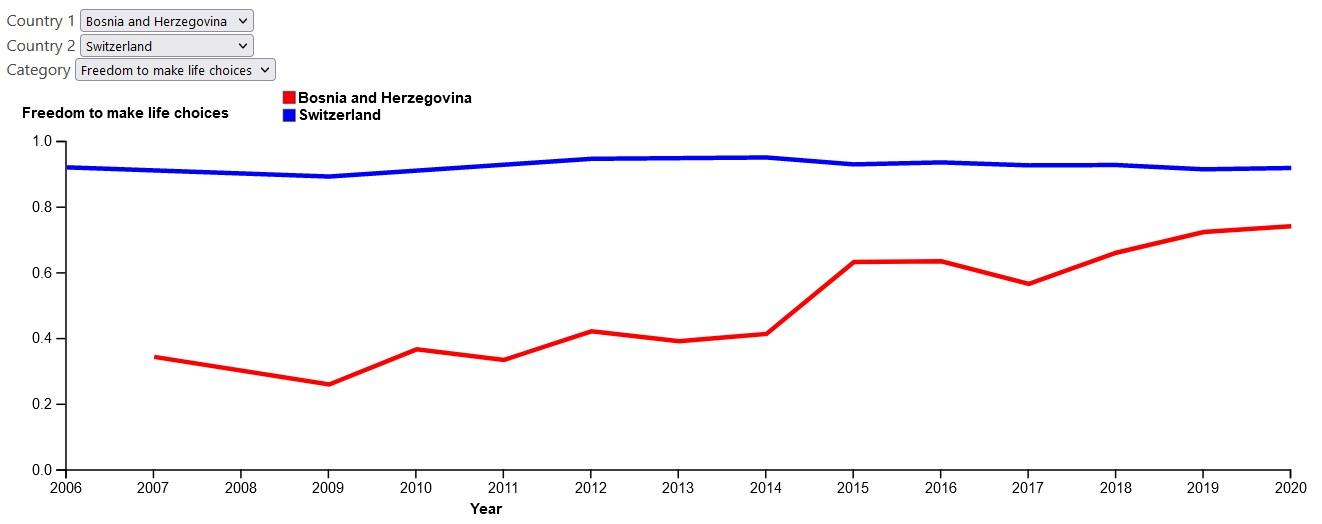
\includegraphics[width = \textwidth]{img/timeseries_anw.jpg}
 \caption{Zeitreihen Vergleich}
 \label{fig:time_anw}
\end{figure}

Wie hier in Abbildung.\ref{fig:time_anw} zu sehen sind die Beständigkeit der Werte und Entwicklung unterschiedlich für die ausgewählten Länder, Schweiz und Bosnien Herzegowina. Die hier ausgewählte Größe ist die Freiheit Entscheidungen zu treffen. Diese liegt in der Schweiz seit 2006 bereits bei ca. 0,9. Das bedeutet fast niemand in der Schweiz hat das Gefühl in seinen Lebensentscheidungen eingeschränkt zu sein. Für Bosnien Herzegowina sieht es etwas anders aus, die Daten starten in 2007 mit ca. 0,4 und enden 2020 bei ca. 0,7. Das heißt das in 2007 sich noch knapp über die Hälfte der Bevölkerung eingeschränkt fühlt während es 2020 nur noch unter ca einem Drittel dieser Auffassung sind. Hier ist eine Entwicklung deutlich zu erkennen. 